Convolution Neural Network (CNN) คือโมเดลปัญญาประดิษฐ์ประเภทหนึ่ง ซึ่งมักจะนำมาใช้กับงานที่เกี่ยวข้องกับรูป โดยการดึงจุดเด่นของภาพออกมา เพื่อใช้สำหรับการจำแนกประเภทของสิ่งต่าง ๆ

\begin{figure}[!ht]
	\centering
	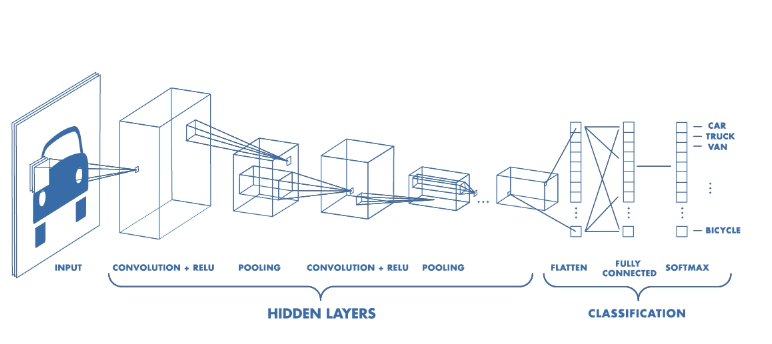
\includegraphics[width=1\textwidth]{chapter2/images/CNN.png}
		\caption{ตัวอย่างโครงสร้างของ CNN}
    	\label{fig:CNN architecture}
\end{figure}

ซึ่งการคำนวณ CNN นั้นจะเริ่มจากการแยกคุณลักษณะออกมาจากรูป โดยการใช้เคอร์เนล (kernel) ซึ่งการที่เคอร์เนลมีลักษณะไม่มีเหมือนกันนั้น จะทำให้คุณลักษณะที่ดึงออกมาจากรูปแตกต่างกัน โดยปกติแล้วเคอร์เนลจะมีหลายแบบ เพราะ ใช่สำหรับการหาคุณลักษณะที่มีรูปแบบต่าง ๆ รูปแบบของเคอร์เนลจะเป็นตารางสองมิติที่มีขนาดขึ้นอยู่กับผู้สร้างที่จะออกแบบ รูปด้านล่างจะเป็นรูปตัวอย่างของเคอร์เนล

 \begin{figure}[!ht]
	\centering
	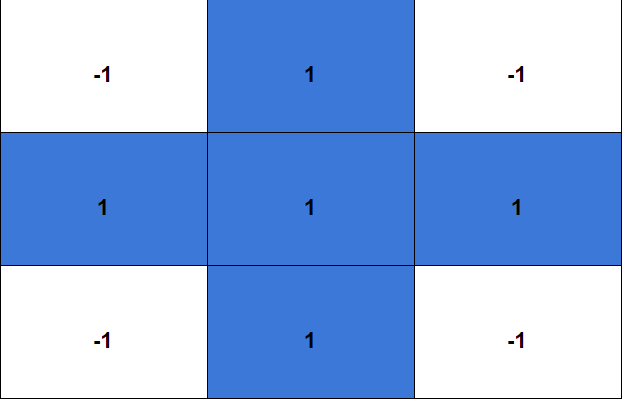
\includegraphics[width=0.5\textwidth]{chapter2/images/kernel_3x3.png}
		\caption{ตัวอย่างเคอร์เนล }
    	\label{fig:CNN architecture}
\end{figure}
\clearpage
เมื่อนำเคอร์เนลไปทาบกับรูปจะทำให้สามารถดึงคุณลักษณะออกมาได้ และเลื่อนตัวเคอร์เนลไปยังพิกเซลต่อไปจนครบทั้งรูป ซึ่งการเลื่อนนั้นขึ้นอยู่กับผู้สร้างว่าต้องการจะให้เลื่อนเท่าไหร แต่ระยะการเลื่อนที่มากขึ้นจะทำให้ความเกี่ยวข้องของคุณลักษณะที่ได้ออกมาน้อยลงด้วย โดยการวางเคอร์เนลเทียบบนรูปนั้นจะวางเคอร์เนลไม่ไห้เกินกรอบรูป แต่ถ้าต้องการทาบเคอร์เนลกับทุกพิกเซลในรูป สามารถทำได้โดยการพื้นที่เกินขอบรูปเท่ากับ 0 ได้ เป็นต้น คุณลักษณะที่ได้ออกมาทั้งหมดจะเรียกว่าผังคุณลักษณะ ตามรูปด่านล่างดังนี้

 \begin{figure}[!ht]
	\centering
	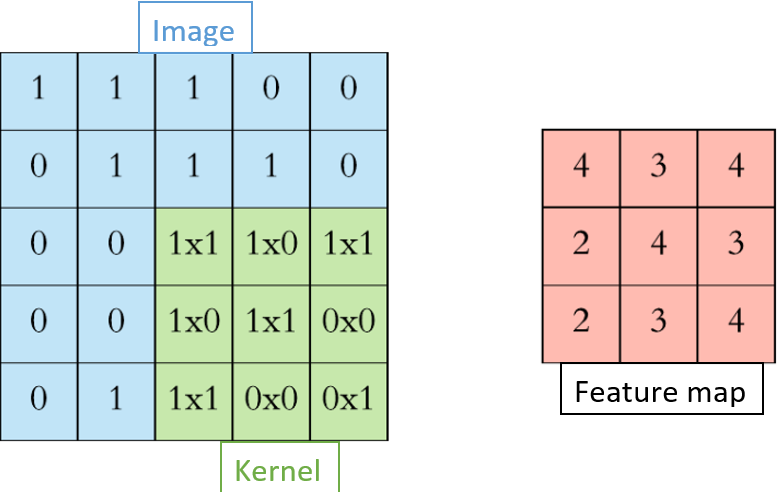
\includegraphics[width=0.5\textwidth]{chapter2/images/feature_map.png}
		\caption{ตัวอย่างการหาผังคุณลักษณะ }
    	\label{fig:example feature map}
\end{figure}

นอกจากนี้การทำเคอร์เนลยังมีการทำอีกแบบนึงซึ่งเรียกว่าการทำ pooling มีความสามารถในย่อรูปภาพแบบนึง ซึ่งนิยมใช้กันอยู่สองประเภทได้แก่ max pooling และ average pooling
โดยที่ max pooling เมื่อนำไปทาบกับรูป จะหาค่าที่มากที่สุดออกมา ตัวอย่างตามรูปด้านล่างดังนี้

 \begin{figure}[!ht]
	\centering
	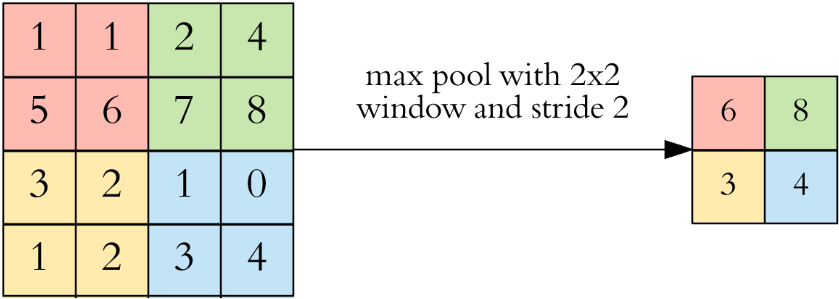
\includegraphics[width=0.5\textwidth]{chapter2/images/max_pooling.png}
		\caption{ตัวอย่างการทำ max pooling }
    	\label{fig:example max pooling}
\end{figure} 

ในขณะที่ average pooling เมื่อนำไปเทียบกับรูป จะหาค่าเฉลี่ยของบริเวณที่เทียบออกมาตามรูปด่านล่างดังนี้

 \begin{figure}[!ht]
	\centering
	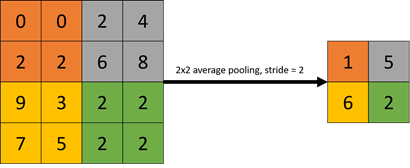
\includegraphics[width=0.5\textwidth]{chapter2/images/average_pooling.png}
		\caption{ตัวอย่างการทำ average pooling }
    	\label{fig:example average pooling}
\end{figure}
\clearpage
ในขั้นตอนการทำนาย ชั้นที่ชื่อว่า Fully connected ในขั้นนี้จะเป็นขั้นที่นิวรอนทุกตัวเชื่อมต่อกัน ซึ่งในงานประเภทตรวจจับวัตถุมักใช้ชั้นนี้ในการทำนายผลความน่าจะเป็นของแต่ละหมวดหมู่ 
 \begin{figure}[!ht]
	\centering
	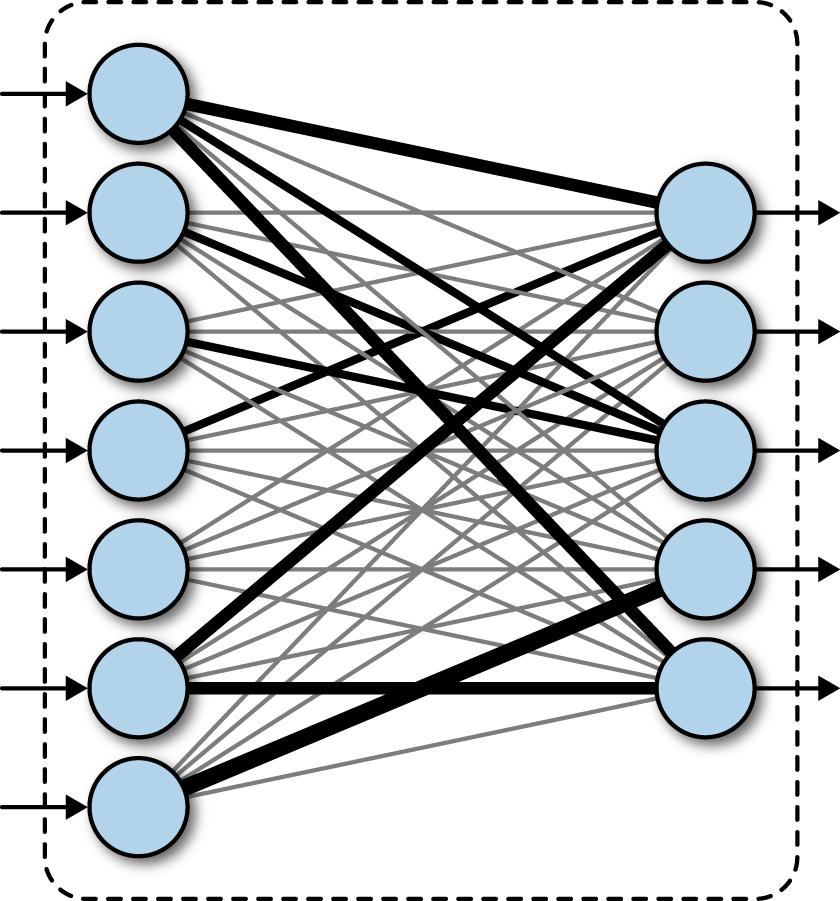
\includegraphics[width=0.3\textwidth]{chapter2/images/fully-connected.png}
		\caption{โครงสร้างของ fully-connected}
    	\label{fig:fully-connected}
\end{figure}
